\section{Evaluation}
First, we investigate the performance of Dynamic Heap Resizer 
(DHR) compared to two static configurations: (1) hand-tuned 
(ideal) and (2) even DRAM division (50-50). 
Figure~\ref{fig:gc_exec_time} depicts the normalized 
execution time of three representative Lucene benchmarks 
(M1, M2, and M3) on the Titan2 server. Within each group,
the first and second columns correspond to static ideal and 
static 50-50 partitioning, respectively, while the third
column represents DHR.

Overall, DHR consistently outperforms both static
configurations across all benchmarks. In particular,
compared to the static 50-50 configuration (even), DHR
achieves execution time reductions of 14.3\% for M1, 15.8\% 
for M2, and 1.3\% for M3. Compared to the hand-tuned (ideal)
configurations, DHR provides performance improvements of 
up to 13.4\% (M2). 
Although DHR improves overall performance, we observe an increase 
in GC time, particularly in M1 and M2. This increase is attributed
to high minor GC activity caused by the creation of many backward 
pointers within these workloads. Backward pointers are references 
from older to younger objects, which prevent objects from being 
collected during minor GCs, resulting in higher promotion rates and
increased GC overhead.

Specifically, GC time nearly doubles in M1 (1.87–1.93× increase) and
increases by approximately 19\% (1.18×) in M2 compared to static configurations. 
In contrast, M3 exhibits a slight decrease in GC time, indicating minimal backward 
pointer impact.


\begin{figure}[htbp]
  \centering
  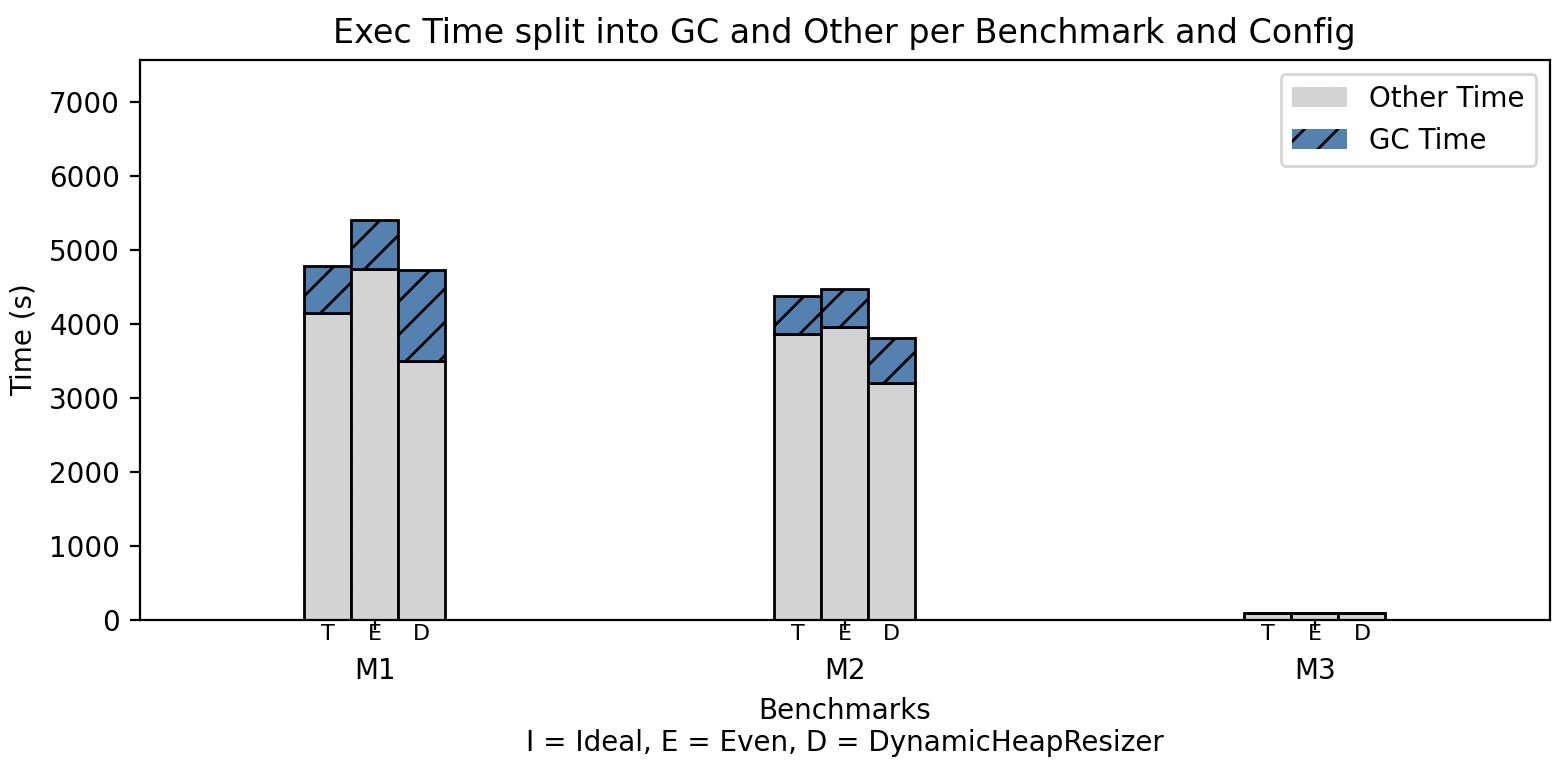
\includegraphics[width=1\columnwidth]{fig/eval_graph.png}
  \caption{Execution time and GC time comparisons}
  \label{fig:gc_exec_time}
\end{figure}

